\setcounter{chapter}{4}
\chapter{Modelling}
\label{chap:modelling}
% 
\section{Introduction}
% 
Nerve fiber modelling is a \dummy, which is \comment{(mainly?)} used in simulations like \ac{dMRI} simulations \dummy.
However most \ac{dMRI} simulation tools use fast simulation techniques as \dummy.
This take analytical function describing the fiber paths to be capable of calculation very fast.
% 
Current algorithm are capable of using spline functions for individual nerve fiber or fiber bundles \cite{Balls2009}.
% 
In resent time with the improvement of computer power and algorithms, simulators like monte carlo are used \dummy.
These simulate the random walk of individual water molecules inside a volume.
If the target are \ac{WM} phantoms nerve fibers can be modelled as a meshed tube.
These have the advantage, that any complex configuration can be modelled \eg beeding fibers \dummy.
\\
%
However, a disadvantage is that for resanable model sizes ( in \ac{dMRI} a voxel is about \SIrange{100}{1000}{\micro\meter} order, size nerve fiber about \SI{1}{\micro\meter}), the number of triangles of the mesh is quite big [\dummy].
A further challange is to build a geometrical configuration, where no nerve fibers are overlapping each other (\ie  take the same volume in space).
\\
% 
Collision detection takes a major role here.
While other simulations which are using geometrical models (\eg protein folding \dummy) can use something like electric potentials, where the actually geometrical boundary is not that important.
As we will we in the case of \ac{3D-PLI} (and \ac{dMRI}) it is different.
\\
% 
Inside this chapter the following procedures are described:
\begin{itemize}[nosep]
    \item geometrical representation of nerve fiber (bundles)
    \item user friendly building methods
    \item ensure collisionless models
\end{itemize}
% 
\paragraph{\ac{fastPLI} modules}
% 
The python sub package \pymodule{fastpli.model} consist of two modules:
% 
\begin{itemize}[nosep]
    \item \pymodule{sandbox}
    \item \pymodule{solver}
\end{itemize}
% 
The first module \pymodule{sandbox} enherets routines to help the user build simple geometric configurations.
Ths can then be used to build more complex structres of nerve fiber bundles.
The second module \pymodule{solver} contains a \CXX framework wrapped inside a \python class to ensure easier user \ac{API} (see \dummy).
\\
% 
First it has to be decided, how to represent a nerve fiber (bundle).
% 
\vspace{5pt}
\hrule
\vspace{6pt}
% 
\section{Nerve fiber representation}
\label{sec:nerve_fiber_representation}
% 
As described in \cref{sec:fiberArchitecture} \ac{WM} consist of densely packed bundles of nerve fibers.
Nerve fibers themselves consist of axons surrounded by myelin (see \cref{fig:nerveFiber}).
The myelin is further split into several parts separated by Ranvier nodes to allow the spread of an action potential.
In the central nervous system, myelin is produced by olegodendrocytes, which are cells that wrap with their little \say{arms} around axons that are locally adjacent.
The wrapping substance is called myelin and consists mainly of a lipid (fat) substance.
\\
% 
The Question is, how to model/represent this tissue?
\\
% 
The main focus of the modelling is to ensure that these models can be used for \ac{3D-PLI} simulations.
However, it is reasonable that these models can also be used for other tasks \eg for \ac{dMRI} simulations.
% 
\paragraph{What does usable mean?}
Since we are working with simulations, the computer algorithms have to be capable of getting an input for a geometrical fiber architecture.
An obvious candidate are used in visualisation techniques.
There, objects of different shape have to be represented so that the computer algorithm can use the representation to visualise an image of the objects.
An obvious model for a fiber is a tube.
Usually objects like tubes are visualised with a surrounding mesh.
Meshes have the advantage, that a texture can be applied to the surface.
However since meshes consist usually of 3d triangles, this means for a good approximation a lot of points, \ie data/memory, to represent a model.
But even in the visualisation domain tubes are not modeld from inital meshes.
They get initialised by a trajectory, which then gets an additional radius to get a volumetric representation.
This representation can be used as well for nerve fiber tissue.
\\
% 
Already existing techniques \dummy allow to represent such structures as analytical mathematical objects \eg a parametric function $f(t) -> (x,y,z,r)$ with $(x,y,z)$ as 3d coordinate and $r$ as radius.
This however limitates the use drastically, since the user has to know in advance a parametic function.
For trivial structures like parallel straight fibers this is quite easy and fast to process.
However, if we want to model more complicated tissues like densly interwoven fiber bundles, the task is nearly impossible.
One possibility would be to do not care, if two fibers overlap, \ie take the same space in volume.
This is done \eg for simulations like protein folding, where the main interaction comes from electro dynamical forces.
However it could already be shown, that for more complicated \ac{3D-PLI} simulations like \dummy non overlapping fibers are essential.
\\
% 
For this reason it was decided to represent fibers in such a way that it will later be able to easily check for colliding objects, \ie nerve fibers.
This means that the number of objects have to be small, with respect to the approximation of the desired level of detail.
A second feature is that the chosen geometries have to be fast calculable for collision detection with each other.
\\
% 
\begin{figure}[!t]
    \centering
    \def\tikzwidth{0.75\textwidth}
    \inputtikz[true]{gfx/model/conical_capsule_bb}
    \tikzset{external/export=false}
	\caption[cc and co]{\Acf{CC}: \raisebox{.25em}{\tikz \draw[black](0,0)--(0.275,0);} \ac{CC}, \raisebox{.25em}{\tikz \draw[blue, dash pattern=on 2.5pt off 2.5pt](0,0)--(0.275,0);} capsule, \raisebox{.25em}{\tikz \draw[red, dash pattern={on 2.5pt off 0.9pt on 0.42pt off 0.9pt}](0,0)--(0.275,0);} bounding box}
	\label{fig:conical_capsule}
\end{figure}
% 
To allow a arbitrary level of detail, a tube like fiber can be split into a number of segments.
Each tube segment can than be approximated as a cylindrical object.
However since the radius of the nerve fibers can vary quite a bit along its path, the tube (or fiber segments) has also to be allowed to change.
If this is done via a cylindrical approximation, the boundry effects between two segments can lead to unusually appearance/behaviour.
It was therefore decided to approximate a fiber segment with a \ac{CC}, a 3d cone on which end spheres with the required radii are attached (see \cref{fig:conical_capsule}).
This has the advantage, that between two fiber segments there is a smooth transition along the fiber axis (for a reasonable curvature) (see \cref{fig:fiberReb, fig:model_length}).
% 
\begin{figure}[!t]
    \def\tikzwidth{0.85\textwidth}
    \centering
    % \tikzset{external/export next=false}
    \inputtikz[true]{gfx/model/fiber_model}
	\caption[]{representation of nerve fiber from a list of spheres $\left\{ \vv{p}_i=(x_i,y_i,z_i), r_i \mid i \in \{0,1,N_{\mathit{points}}-1\}\right\}$.}
	\label{fig:fiberReb}
\end{figure}
% 
A nerve fiber can therefore be represented as a list of 4d coordinates (or spheres) (see \cref{fig:fiberReb}):
% 
\begin{align}
\begin{split}
% \vv{p} &= (x_i,y_i,z_i) \mid x,y,z \in \mathbb{R}\\
% r &\mid r \in \mathbb{R}\\
\mathit{fiber} &= \left\{ \vv{p}_i=(x_i,y_i,z_i), r_i \mid x,y,z \in \mathbb{R}, \, r \in \mathbb{R^+}, \, i \in \{0,1,...,N_{\mathit{points}}-1\}\right\} \\
\mathit{fiber\_seg}_i &= (\vv{p}_i, \vv{p}_{i+1}, r_i, r_{i+1}), \, i \in \{0,1,...,N_{\mathit{points}}-2
\end{split}
\end{align}
% 
\section{Sandbox}
% 
Since the geometric representation of the fibers is defined, the question arises how such fibers can be constructed.
For this purpose the \ac{fastPLI} module \textit{fastpli.model.sandbox} was developed.
It contains a variate of methods to allow the user fast building algorithms to generate complex phantoms.
\\
% 
These Algorithms can be split into two parts.
Since this toolbox concentraits to prepair phantoms for the \ac{WM}, the focus on building also n buolding such structures.
Since \ac{WM} nerve fiber bundles are usually combined into nerve fiber bundles (see \dummy), the \textit{sandbox} module contains two major parts o buld exatly such structures.
%
Nerve fiber bundles can be represented in a similar way as nerve fibers: tube like structures populated with individual nerve fibers.
How to represent tube structures was already accomplished (see \cref{sec:nerve_fiber_representation}).
\\
If we think of nerve fiber bundles as a trajectory through the 3d coordinate systems, we can use the same representation as of nerve fibers.
Additionally the contained radii can be used to scale a nerve fiber along its trajectory, \ie to inflate it.
\\
% 
The question remains, how to \say{populate} such bundles.
To populate a trajectory we can use a similar approach to tractography (see \cref{sec:fillBundle}).
We start with seed points at the beginning of the bundle.
\todo{improve transition}
% 
\subsection{Seeding a nerve fiber bundle}\label{sec:seeds}
% 
\begin{figure}[!t]
    \def\tikzheight{0.25\textwidth}
    \centering
    \subcaptionbox{\label{fig:triGrid}equilateral triangle grid}[.295\textwidth]{
    \inputtikz{gfx/model/triangular_grid}\hfill}
    \subcaptionbox{\label{fig:rndGrid}random grid}[.295\textwidth]{
    \inputtikz{gfx/model/rnd_circle_points}}\hfill
    \subcaptionbox{\label{fig:crossBundle}populated fiber bundles}[.39\textwidth]{
    \inputtikz{gfx/model/crossing_bundle}\hfill}
	\caption{Populating fiber bundles with seed points.}
% 	\label{fig:}
\end{figure}
% 
The initial seed can already determine specific outcomes of nerve fiber bundle geometries. 
They are stored as a list of 3d points:
\begin{align}
\mathit{seeds} = \left\{ \vv{p}_i=(x_i,y_i,z_i) \mid x,y,z \in \mathbb{R} , \, i \in \{0,1,N_{\mathit{seed\_points}}-1\}\right\}
\end{align}
% 
To build escepcially dense fiber bundles, a method to generate a equiliteral triangular grid was implemented.
Mathematically a 2d packed circle contains the maximum package density if it is arrange in a triangular (or sometimes called hexagonal) grid for circles with equal radii (see \ref{fig:triGrid}).
This highly regular symmetrical grid can however lead later to strange results in simulations (\eg maxwell, simpli).
\todo{why rnd necesarry -> see simulation}
Therefore it should only be uses as a initial configuration. 
The positions can easily modified.
A useful method was to add a rand value to the initial seed points, \eg $\mathit{shift} = norm(0,\sigma)$.
However since the initial configuration is often unknown, it would be probably best to choose a random distribution.
For a circle this is done via:
\begin{equation}
\begin{aligned}
 \varphi &= \mathrm{uniform}(0,2 \pi) \hspace{4.2ex} && x = r \cos(\varphi)\\
 r &= R \sqrt{\mathrm{uniform}(0,1)} && y = r \sin(\varphi)
\end{aligned}
\end{equation}
% 
\subsection{Populate bundles}\label{sec:fillBundle}
% 
\begin{figure}[!t]
    \centering
    \subcaptionbox{\label{fig:torsionCurve}Torsion along trajectory. The 
	\textcolor{green!50!black}{binormal}, \textcolor{red}{principal normal} vector and \textcolor{blue}{tangent vector} vector at each step are also the coordinate system for the seed points.}[.5\textwidth-1ex]{
    \def\tikzwidth{0.5\textwidth-1ex}
    \inputtikz[true]{gfx/model/min_torsion}}\hfill
    % 
    \subcaptionbox{\label{fig:filledBundle}Bending fiber along trajectory $f(t) = \left( \cos(t), \sin(t), 0 \right)$}[.5\textwidth-1ex]{
    \resizebox{0.5\textwidth-1ex}{!}{
    \includegraphics{dev/gfx/circle_bundle.png}}}
	\caption{}
% 	\label{fig:}
\end{figure}
% 
To populate a nerve fiber bundle, the same idea as in tractography is used.
There, seed points are initialized, and then via \dummy methods a next step is calcuulated.
However, we don't need to calculate the next step, sinice it is already defined by its trajectory.
However, the bending of the bundle has to be taken into account.\\
% 
Here, different techniques already exists.
A common one is to use the torsion of the curve. This is achieved via the following method:
% 
\begin{align}
\begin{split}
\vv{f}(s) &= (x(s),y(s),z(s)) \\
\vv{t}(s) &= \vv{f}\,'(s) \\
\vv{n}(s) &= \frac{\vv{t}\,'(s)}{|\vv{t}\,'(s)|} = \frac{\vv{r}\,''(s)}{|\vv{r}\,''(s)|} \\
\vv{b}(s) &= \vv{t}(s) \times \vv{n}(s),
\end{split}
\end{align}
% 
where $\vv{f}(s)$ is a parameterised trajectory of the parametric variable $s$, $\vv{t}(s)$ the tangential vector, $\vv{n}(s)$ the principal normal vector and $\vv{b}(s)$ the binormal vector (see \cref{fig:torsionCurve}).
One could use this idea to rotate the seed points into the coordinate system of $\vv{t}(s),\vv{n}(s),\vv{b}(s)$.
However this can lead to a arbitry rotation of the fibers, \eg when the curve descibes such a way that $\vv{n}(s),\vv{b}(s)$ would continous rotating around $\vv{t}(s)$.
\\
% 
Since it is plausible, that nerve fiber bundles would not do this, a different approach was decided.
The idea is, to minimise the rotation from one step to the next step.
% If the trajectory, \ie nerve fiber bundle is at step $i$, it came form $i-1$ and goes to $i+1$.
% Therefore one can describe a perpendicular plane between this points:
If we define a plane, inside the above define vectors $\vv{n}(s),\vv{b}(s)$ we want that from one step $i$ to the next step $i+1$ the plane is rotated by the same amount as the curve bends.
However the rotation along the vector $\vv{t}(s)$ shell be $0$.
Since we have a discrete points, we can therefore rotate the plane with the same amount, as the vector $\vv{t}(s)$ obtains.
However to optain a plane in the \say{middle} of the points $\vv{p}_{i-1}, \vv{p}_{i}, \vv{p}_{i+1}$ we will use the mean orientation of these points.
An example is shown in \cref{fig:filledBundle}.
\\
\todo{explain and check algorithm}
% 
Now the populate of the bundle can simply full filled by starting a the beginning of the fiber, placing the seed points at the start point, and rotating the seed point for each step $i$ along the trajectory by only rotating along one vector perpendicular to the curve bending.
% 
\subsection{cube models}
% 
\begin{figure}[!t]
    \centering
    \def\tikzwidth{0.75\textwidth}
    \inputtikz{gfx/model/cube_build}
	\caption{Populating a cuboid with straight fibers initialized from seed points along the direction $\vv{v}$.}
    \label{fig:cubeBuild}%
\end{figure}
% 
To be able to generate a model with a main fiber orientation, a method to populte a cuboid volume was developed as well.
This method allows to generate fibers inside the cuboid volume which are orientated along a user given main orientation $\vv{v}$ (see \cref{fig:cubeBuild}). 
The individual fibers are initialized with seed points as well.
A infinity line will be placed through each seed point with the main orientation $\vv{v}$.
If a line is colliding with the volume, the line inside the cuboid is returned as a fiber.
% 
\subsection{cylindric models}
% 
\begin{figure}[!t]
    \centering
    \def\tikzwidth{0.31\textwidth}
    \subcaptionbox{\label{fig:cylCircular}%
        \dummy.
    }[.33\textwidth-1ex]{
    \inputtikz{gfx/model/cylinder_circular}}\hfill
    % 
    \subcaptionbox{\label{fig:cylRadial}%
        \dummy.
    }[.33\textwidth-1ex]{
    \inputtikz{gfx/model/cylinder_radial}}\hfill
    % 
    \subcaptionbox{\label{fig:cylParallel}%
        \dummy.
    }[.33\textwidth-1ex]{
    \inputtikz{gfx/model/cylinder_parallel}}
	\caption{The green area indicates the surface corresponding to the seed points xy-plane. The \textcolor{red}{red} coordinate system indicates the coordinates origin for the seed points.}
% 	\label{fig:}
\end{figure}
% 
Finally a method to build cylindrical structures was implemented as well.
Since a cylinder has three symmetries, all three were implemented to be a option to populate the volume.
First we define the coordinate system.
The cylinder of an outer radii $r_{\mathit{out}}$ and inner radii $r_{\mathit{in}}$ will be orientated along the z-axis with a height $h$, starting at $(0,0,0)$.
Additionally the cylinder can be radial be \say{cut} from a directional angle $\alpha$ to $\beta$.
% 
\paragraph{a) circular} mimics a path on the $xy$-plane of a cylinder (see \cref{fig:cylCircular}).
The seed points will be used along the surface of cross section beginning at the first directional angle $\alpha$.
From there the fibers path will go along circular until the second directional angle $\beta$.
The step size of the circular path can be changed.
% 
\paragraph{b) radial} cylindric fibers are orientated from the center of the $xy$-plane the outside of the cylinder (see \cref{fig:cylRadial}).
The seed points are localized along the inner radial plane.
This way the fiber density will decrease along their path.
% 
\paragraph{c) parallel} fibers are orientated along the cylinder (see \cref{fig:cylParallel}).
Here the seed points are in the $xy$-plane. Only fibers will be used, which are colliding with the cylinder.
% 
\section{Solving fiber collisions}
% 
One major drawback of all previous methods is, that the user has to make sure, that his fiber trajectory let enough space, so that the fibers (trajectories + radii) have enough space and do not intersect with each other.
This maybe achievable for fibers with constant radii along there path for the upper construction methods.
However, for more slightly more complex structures, \eg crossing fiber bundles, this already is nearly impossible.
Therefore a method was developed, which takes the user defined fibers and checks them for collisions.
When a collision is found it will try to move the colliding objects slightly apart, so that the collision will start to disappear.
\\
% 
This concept is rather simple.
The algorithm for collision detection are already used for century's especially in gaming world, where a character \eg should not be capable to walk through a wall. Another wide verity of algorithms are used in visualisation. There usually the problem is to detect the collision between a light path (mathematical line) and a object, usually a triangular surface. Also known as ray tracing.
The drawback in both fields is, that computing time is limited.
Therefore there algorithms use shortcuts as close to reality as possible but still produce usable data. \eg in computer games it is very important to have a stable frame rate of above $\num{60}$ \ac{fps} (or with the current technology even above 120 \ac{fps}).
However it does not matter much for the gaming experience, if the character can walk slightly into a object or not.
Therefore an object like a stone could be approximated by a sphere(s).
\\
%
However since here we want to generate as good as possible large, complex and precise models, a new algorithm has to be developed which is specialised in this subject.
% 
\\[\baselineskip]
% 
For this purpose an algorithm was developed and publish in \cite{matuschke2019}.
It is at this point integrated inside the \ac{fastPLI} package under \pymodule{fastpli.model.solver}.
It structure consist out of the following parts:
\begin{itemize}
\item main loop
\begin{itemize}
    \item octtree separation
    \item collision detection
\end{itemize}
\item moving objects
\item apply boundary conditions
\end{itemize}
% 
Before we go into the details of the algorithm, first we descipe the collision detection approuch.

\subsection{Collision Detection}
% 
As it was described in \cref{sec:nerve_fiber_representation} nerve fibers are represent as a chain of spheres, where two neighbouring spheres are combined into a fiber segment forming a \ac{CC} (see \cref{fig:conical_capsule}).
% 
Therefore an algorithm is necessary to calculate a collision between to \ac{CC}.
This is a non trivial task and very computational heavy.
Therefore it was decided to change the object representation for the collision detection part from a \ac{CC} to a Capsule (see \cref{fig:conical_capsule}).
This means, that the radii of the \ac{CC} grows for both spheres to the max of both spheres $r_{\mathit{capsule}} = \mathrm{max}(r_0, r_1)$.
This has the disadvantage, that at intersections between two neighbouring cones the radii can be actually smaller, however if the change in radii is not rapid, it is justifiable.
\\
The algorithm to detect collisions between two capsules is shown in \cref{alg:pseudocodeCollisionDetection}:
\\
% 
\setbox0=\hbox{%
\begin{minipage}{0.49\linewidth}
\lstinputlisting[style=cpp, basicstyle={\tiny\ttfamily}, firstline=1,lastline=42]{code/collision_detection.cpp}
\end{minipage}}\savestack{\listingA}{\box0}
% 
\setbox0=\hbox{%
\begin{minipage}{0.49\linewidth}
\lstinputlisting[style=cpp,basicstyle={\tiny\ttfamily}, firstline=43,lastline=84,firstnumber=43]{code/collision_detection.cpp}
\end{minipage}}\savestack{\listingB}{\box0}
% 
% \begin{landscape}
\begin{sideways}
\begin{tabular}{|c|c|}
\hline
\stackinset{l}{}{}{}{}{\listingA} &
\stackinset{l}{}{}{}{}{\listingB} \\
\hline
\end{tabular}
\end{sideways}
% \end{landscape}
% 
\subsection{Octtree}
% 
This means that a collision algorithm has to check all existing fiber segments with each other.
It is trivial to see that the computational effort grows with $\mathcal{O}(n^{2})$ which is not acceptable for large $n$.
% 
% 
% 
\vspace{5pt}
\hrule
\vspace{6pt}
% 
\newpage
% 
% 
% 
This Method aims to model den sly \ac{WM}.
The main component inside \ac{WM} consist of an Axon and its surrounding Myeling [see \dummy].
The Myelin itself is split into several parts to allow the propagation of the action potential at the Nodes of Ranvier. 
\\
% 
This structure is modelled as a chain of capsules, a cylinder with hemispherical ends \cref{fig:conical_capsule}.
To allow a change of cross section or radii, the capsule ending are allowed to consist of individual radii.
The resulting shape will be referred to as a \ac{CC}.
The chain of \ac{CC} consist therefore of a list of 3d points with individual radius. 
\\
% 
To model flexible and curved densly packed nerve fibers, a collision free result needs to be obtained.
The representaion of nerve fibers by \ac{CC} allows a fast calculation if two \ac{CC} are colliding each other. 
\\
% 
However instead of building a collision free model, which is quite impossible for a \dummy structure, the strategy is to initialize a model, checking for collisions and then solving these collisions by pushing the fiber or \ac{CC} slightly apart. 
\\
% 
This allows a user to specify any initial configuration and reaching a collision free model, which, depending on the initial overlap, follows the initial geometry.
The disadvantage obvious is that the configuration has to change.
However since biological tissue is deformable and not "caotic" itself, it follows its natrual behavier.
%
% 
% 
% 
Collision detection for a large number of objects is a very computational intense algorithm.
To reduce the computational afford, the \ac{CC} will be interpreted as a capsule object, since this alows a much simpler calculation.
The capsule has the radius $r_{\text{capsule}} = \max(r_0, r_1)$ to soroun the hole \ac{CC}.
To check if two capsules collide with each other the distance between the line segments, defined by the capsule begin and end points $p_0, p_1$, is calculated.if the distance $d$ is $d < (r_0 + r_1)$ then the two capsule objects are colliding each other. \\
% 
To calculate the smallest distance between two line segemnts, sevverel algorith,s already exists.
A fast approach was chosen\footnote{\href{https://www.john.geek.nz/2009/03/code-shortest-distance-between-any-two-line-segments/}{https://www.john.geek.nz/2009/03/code-shortest-distance-between-any-two-line-segments/}}.
%
\section{World}
For a given cuboid volume the computing grows $\mathcal{O}(V^3)$.
Furthermore each object has to be checked to each other, therefore the number of objects to be checked for a collision grows by $\mathcal{O}(n^2)$.
This explodes rather quick.
In the literature are several approuches (e.g. computer games industry).
However since the number of objects will be $\approx \num{e9}$ \dummy cant be used. \\
% 
A "tree" is a data structure consist of a collection of "nodes", which are connected to each other.
One node is conected toword the "root" with a single parent node and towords the "branches" with several "children" or "branches".
The nodes at the end of a branch are refered to as "leafs" wich contain the data.
Traversing a  evenly distributed tree is of $\mathcal{O}(\log(n))$.\\
% 
\begin{figure}[!t]
    \centering
    \subcaptionbox{oct tree}[.3\textwidth]{
    \def\tikzheight{0.6\textwidth}
    \inputtikz{gfx/model/oct_tree}}
    \subcaptionbox{collision 2d}[.65\textwidth]{
    \def\tikzheight{0.6\textwidth}
    \inputtikz[true]{gfx/model/collision_tree}}
	\caption{}
	\label{fig:oct_tree}
\end{figure}
% 
An octtree is a special kind of tree where each node contain 8 children.
This allows to divide a cubic volume into 8 equal cutted subcubes.
Therefore this data structure was chosen to reorder the fiber segents.
To order them, a recursive function is used.
It checks, if the number of objects is below a threshold $n < t_n$, or the subvolume cube length is below a threshold $dim < t_{dim}$.
If so, the leaf is reached and all objects are check for collision with each other.
Otherwise a 8 new subvolumes will be created and each object will be check, if it is inside upto 8 of the new created volumes.
The next branch will check only with the new includes objects. \\
% 
This allows a rather quick reduction of number of objects to be checked.
Therefore the last step with an $\mathcal{O}(n^2)$ is not that painful anymore.
To speed up the calculation, The objects itself wont be duplicated.
All objects are contained in a \textit{std::vector} of cones.
Only the indices will be transfered to the next recursive function call.
Also the objects are traversed in order, so that the maximum speed from the cpu cache can be exploited. \\
% 
The minimal subvolume size is choses to $\sqrt{3} \times \max(\mathit{object\_size})$.
Smaller then this would only replicated subvolumes with identical contained objects.
The maximum number of objects is set to \num{25} objects \footnote{found suitable by testing.}. \\
% 
The building of the tree is don in parallel.
Up to 8 threads are spawned to check for the first 8 subvolumes, which objects are contained.
The next level can again spawn upto 8 new threads (64 in total).
This compensates if a the objects are not uniformly distributed.
After the first level, each cpu thread traverses it branch.
At each leaf a list ob object is returned containing the object of the leaf.
All list are collected for the collision checking test.
This collected list is in the next step fully parallel traversed to check for collisions.
% 
\section{Solving a collision}
To solve a collision between two \ac{CC} objects the two points of each object will be moved.
The movement will be parallel to the smallest distance line between both objects.
To take the 3d placement into consideration, the movement is weighted with the distance of the the individual points to the intersection point with the smallest distance line (see fig \dummy).
This will result in a more controlled movement if \eg only the two endings of the fiber objects collide each other. \\
% 
The movement is saved for each object in a velocity \textit{std::vector}.
Therefore the sum of all velocities is taken into account.
The maximum speed is however limited to a value of $v_{\max} = 0.1 \times \min(\mathit{object radius})$.
This prevents movement through another object.
% 
\section{Shape Control}\label{chap5:ShapeControl}
The movement of individual points can results in a "distorted" fiber model, \eg two points move very far apart from each other.
Therefore boundry conditions have to be specified.
It was decided to use the following two conditions:
% 
\subsection{Mean segment length}
% 
\begin{figure}[!t]
    \centering
    \def\tikzwidth{.45\textwidth}
    \subcaptionbox{merge}[.49\textwidth]{
    \inputtikz[true]{gfx/model/model_merge}}
    \subcaptionbox{split}[.49\textwidth]{
    \inputtikz[true]{gfx/model/model_split}}
	\caption{Length control for fibers $f$ and $f'$}
	\label{fig:merge_split}
\end{figure}
% 
% 
\begin{figure}[!t]
    \centering
    \def\tikzwidth{0.75\textwidth}
    \tikzset{external/export next=false}
    \inputtikz[true]{gfx/model/model_length}
	\caption{different fiber segment length.}
	\label{fig:model_length}
\end{figure}
% 
The Mean segment length coresponts to the distance between the two points of an object.
If the lenght of the object becomes to small/big, the points inside a fiber coresponding to the object are merged/splitted resulting in one point less / adding a new point.
The minimum/maximum distance of the object is set to $d_{\min} = \frac{2}{3} \overline{d}, d_{\max} = \frac{4}{3}\overline{d}$.
Therefore the mean allowed value of the object is:
\begin{align}
\frac{d_{\min} + d_{\max}}{2} = \overline{d}
\end{align}
% 
If a new point is created due to exceeding the maximum limitation, the new points position $\vv{p}_{new}$ is 
\begin{align}
\begin{split}
\vv{p}_{new} &= \frac{\vv{p}_{i} + \vv{p}_{i+1}}{2}\\
r_{new} &= \frac{r_{i} + r_{i+1}}{2}\\
\vv{v}_{new} &= \frac{\vv{v}_{i} + \vv{v}_{i+1}}{2}
\end{split}
\end{align}
with a radius of $r_{new}$ and a velocity $\vv{v}_{new}$.
% 
\subsection{Bending radius}
% 
The bending radius is defined as the circular radius corresponding to the circle defined by three neighbouring points $p_{i-1}, p_{i}, p_{i+1}$. 
The limit is set as a minimal radius of $r_{\min}$.
If a point $p_{i}$ in a fiber fall below this value, the three points will be moved.
$p_{i-1},p_{i+1}$ will be moved \dummy and $p_{i}$ oposit.
Therefore the curvature will be reduced.
% 
\begin{figure}[!t]
    \centering
    \def\tikzheight{.40\textwidth}
    \subcaptionbox{Boundry segment length: lower bound $phi=\SI{60}{\degree} \xrightarrow{} r_{min} \geq \SI{0.5773}{} \cdot l_{mean}$}[.475\textwidth]{
    \inputtikz{gfx/model/model_circle}}\hfill
    \subcaptionbox{Boundry segment radii: lower bound $r_{min} \geq \fiberRadiusMean $}[.45\textwidth]{
    \inputtikz{gfx/model/model_circular}}
	\caption{Geometrical boundry condition for fiber segment length \segLength and fiber bending radius \segRadius.}
	\label{fig:model_circle}
\end{figure}
% 
\newline
Both movements are added to the velocity vector before performing the overall movement.
The algorithm performs each step sequentially (see \cref{alg:pseudocode_solver}).
\begin{lstfloat}[!tb]
\lstset{style=cpp}

\begin{lstlisting}[]
FiberCollisionSolver(objects) {
	colliding_list = {};
	do{
		// Reset Parameter
		colliding_list.clear();
		SetSpeed(objects, 0);
		
		// Building Octree
		octree = OctTree(objects);
		
		// Collision Detection
		for ( leaf : octree ){
			colliding_objs = CheckLeaf(leaf.fiber_list());
			colliding_list.insert(colliding_objs);
		}
		
		// Seperation Process
		AddSpeed(colliding_list);
		NormalizeSpeed(colliding_list);
		MoveObject(colliding_list);
		
		// Shape Control
		SegmentLength(colliding_list, target_length);
		BendingRadius(colliding_list, target_curvature);
		
	} while (!colliding_list.empty());
}
\end{lstlisting}
\caption{Pseudocode of the main algorithm: The function \texttt{FiberCollisionSolver} will loop the followings four steps, which are run in parallel, until no collision are detected anymore: 1. build an \texttt{OctTree} from all objects, 2. \texttt{Collision Detection}, 3. \texttt{Seperation Process} and 4. \texttt{Shape Control}.}
\label{alg:pseudocode_solver}
\end{lstfloat}
% 
Finaly a volume is marked as collision free, if no collision are found and all boundry conditions are fullfiled. 
The voundry conditions can be set to 0 to ignore them.
Additionally a drag value can be set, to reduce the velocity by its factor after each step.
It can help to reach a collision free volume faster, however the density will be significantly reduced.
Therefore the value is to 0 so that after each step the velocity is resetted to $\vv{0}$. 
% 
% 
\section{Visualization}
% 
A visualization tool was written to visualize the fiber configuration. This allows the user a direct feedback (\eg after each step) to tune the initial fiber configuration or boundry condition. It was written in \textit{OpenGL 2}.
% 
\ac{CC} are either renderd via the \textit{gluCylinder} function provided by the \textit{GLUT} library for a rough but fast visualiation. This represents the capsule representation. For a more precise and correct visualization of the \ac{CC}, a self implemented rendering was developet. The outer hull, or mesh, is created as a tube sourounding the fiber with circular orderd poinuts around a fiber point $p_i$ (see \dummy).
% 
From the mesh, vertices and normals are calculated, which are then finaly rendered. To allow a visualization of the inner axon, the myelin hull can also be transperented rendert. This however needs sorted vertices along the z axis (inside the screen). This process takes quite some time, therefore only feasible for screenshoots at this time (see fig \dummy).
% 
\begin{figure}[!t]
    \def\tikzwidth{0.5\textwidth}
    \subcaptionbox{mesh}[0.49\textwidth]{
    \inputtikz{gfx/model/vis_a}}
    \subcaptionbox{vis}[0.49\textwidth]{
    \inputtikz{gfx/model/vis_b}}
	\caption{Generating mesh for visualization.}
	\label{fig:vis_mesh}
\end{figure}
% 
\paragraph{Disclamer}
This is a fast written approuch. Current rendering software uses far more advanced techniques. However this rendering algorithm was written to be a light integrated tool using only the aditional \textit{OpenGL 2} and \textit{GLUT} library.\\
% 
A more advanced Tool, the \textit{FAConstructor} \cite{Reuter2019} was written by Andr'e Reuter in the context of this doctorial research. This tool uses \textit{OpenGl 3} and additional calculation on the GPU. Additionally it allows user defined interactive technique to create a 3d fiber model.
% 
\subsection{Wall opacity}
% 
To be able to visualize axons inside myelinated nerve fibers, the visualisated vertices have to bi invisible.
This however is a complicated task, since know the order of data processing is important.
\dummy.
% 
% 
% 
\section{Medusa}
% 
Additionally to the previous discussed Algorithm (\dummy), the \ac{MEDUSA} algorithm, was developed in a cooperation with the team Neurospin from \ac{CEA} in France \cite{Ginsburger2019}. The targed was to develop an algorithm which can build a library of \ac{WM} tissue. This library should not only contein nerve fibers, but also other cell types like olegodendrocites or astrocytes. These cell types are currently not used in \ac{3D-PLI} routin analysis however in \ac{dMRI} the cell are quite important [\dummy]. Furthermore these cells take up additional volume which results in different nerve fiber configurations.\\
% 
Since this tool aims to build a statistically library, other parameters are chosen for boundry conditions. These parameters are chosen as close as possible from the current \ac{dMRI} models:
\dummy\\
\dummy\\
% 
% Instead of choosing \ac{CC} the fibers and cells are represented as a collection of spheres. This has the advantage that the collision of spheres are more easier to be calculated:
% \begin{align}
%     d < r_i + r_j
% \end{align}
% 
On the other side more spheres  are needed to represent a fiber. There can always be a resulting overlapp which depnding on the usecase, can lead to .. results.\\
% 
Cells are also represented as a collection of spheres, filling out the sum of the spheres volume. \\
%
In this theses cells are disregarded. A full description of the construction with astrocytes and olegodendrocytes can be found in \cite{Ginsburger2019}.
% 
\subsection{Algorithm}
% 
\begin{figure}[!t]
\centering
% \resizebox{0.75\textwidth}{!}{
\def\tikzwidth{0.75\textwidth}
\inputtikz{gfx/model/medusa/medusa_spheres}
% }
\caption{modified from \cite{Ginsburger2019}}
\label{fig:model:medusa_4}
\end{figure}
%
% \begin{figure}[!t]
%     \centering
%     % \resizebox{0.75\textwidth}{!}{
%     \def\tikzwidth{0.75\textwidth}
%     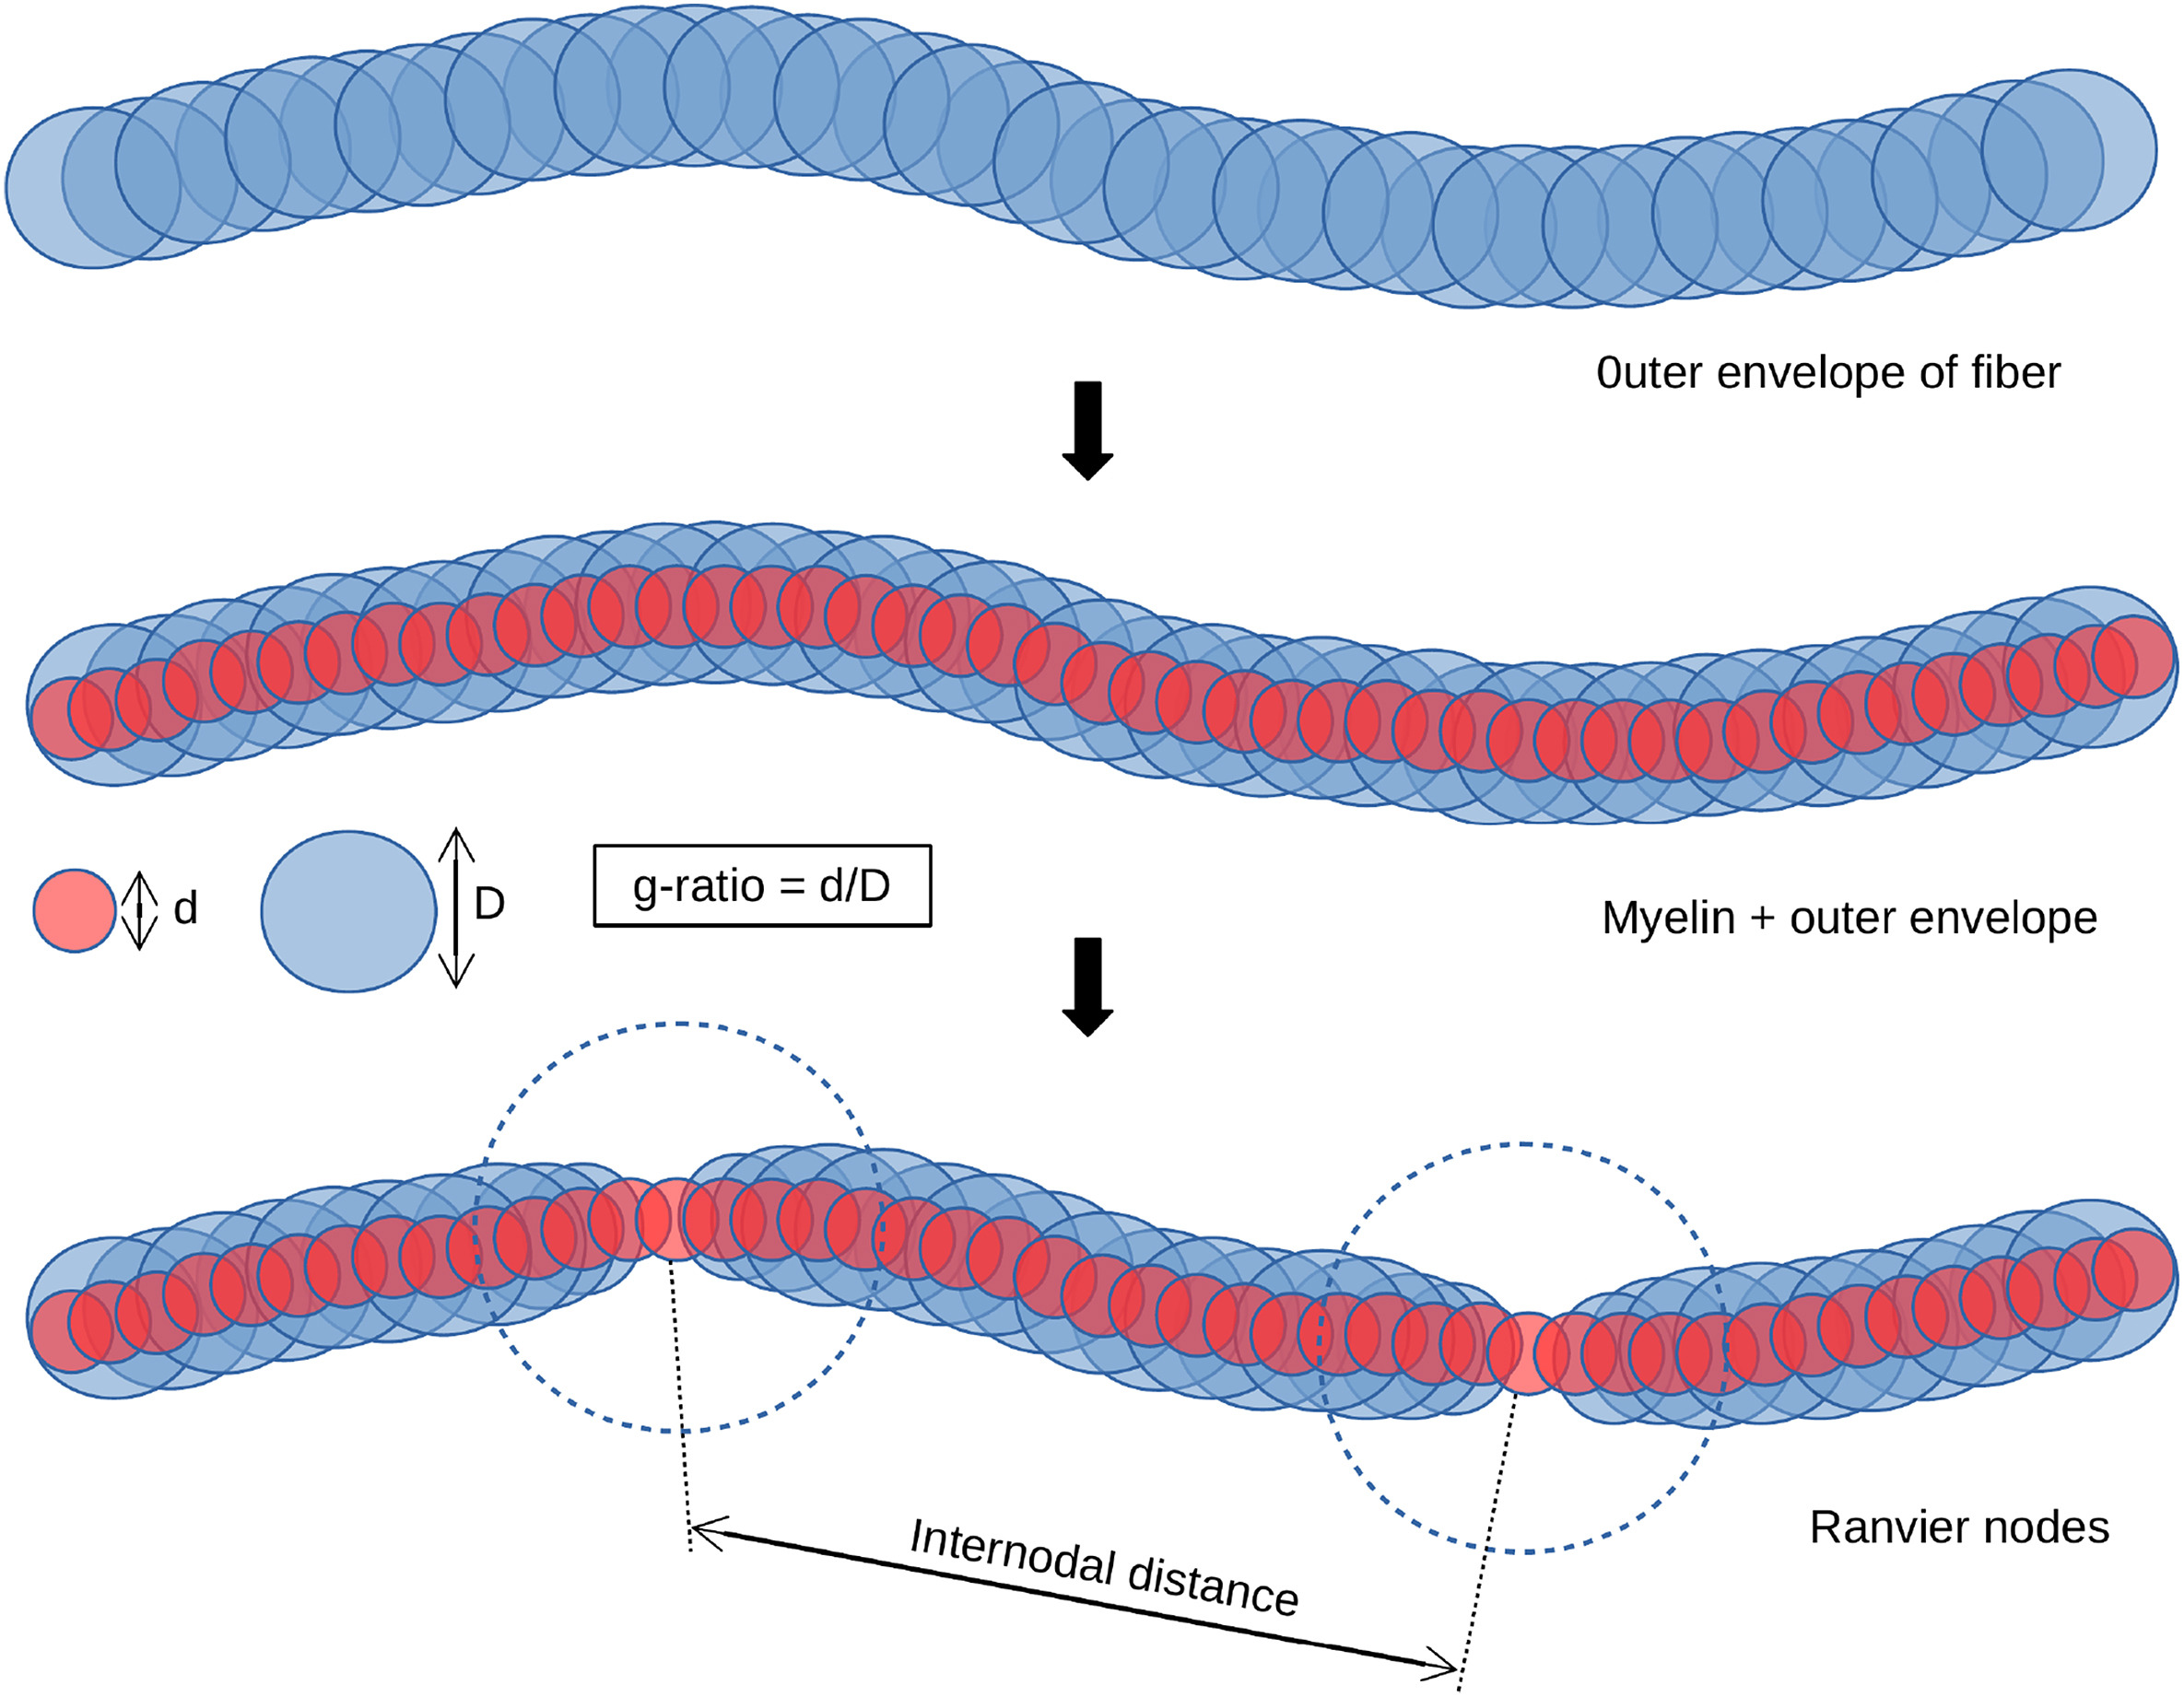
\includegraphics{gfx/model/medusa/4.jpg}
%     % }
% 	\caption{4 \cite{Ginsburger2019}}
% 	\label{fig:model:medusa_4_org}
% \end{figure}
% 
Since all objects are represented as a collection of spheres (see \cref{fig:model:medusa_4})
\begin{align}
    \mathcal{S} = \{ (x_i,y_i,z_i,r_i) : i \in \{0, 1, ..., n_\text{objects}-1\}  \} 
\end{align}
% 
, a collision is present if (VCS !!!)
% 
\begin{align}
\begin{split}
d<r_i+r_j\\
d = \abs{\vv{p}_i - \vv{p}_j}
\end{split}
\end{align}
% 
However since neighboring spheres in one fiber are colliding for a densly populated fiber, they have to be excluded if
\begin{align}
\begin{split}
d(i,j) &\leq  r_i + r_j\\
d(i,j) &= 
\begin{cases}
\sum_{n=i}^{j-1} \abs{\vv{p}_n - \vv{p}_{n+1}},& \text{if } j-i \geq 1\\
0 & \text{otherwise}
\end{cases}
\end{split}
\end{align}
% 
Spheres inside cell bodys are not checked for collision, since their volume aproximate? the volume of the cell.\\
% 
The calculation of collisions is done via the GPU architecture. For this a first implementation was written with the \textit{AxisAligedSortedSearch} \cite{Karras2012}. It sorteds the spheres along one axis, \eg x-axis, and search for each sphere the fist and last possible collision on this axis:
\begin{align}
\begin{split}
\mathcal{C}_i = \{ s \in \mathcal{S} \mid \abs{s_i.x - s_j.x} < r_i+r_j \}
\end{split}
\end{align}
% 
\begin{lstfloat}[!t]
	\lstinputlisting[style=cpp]{code/medusa.cu}
	\caption{Pseudocode of \acs{MEDUSA} collision checking.}
	\label{alg:medusa_collision}
\end{lstfloat}
% 
The above described algorithm is currently used for volumes $\approx \SI{200}{\micro\meter}$. For this volume size the algorithm is for the current use fast enough. However, more advaned algorithm exist wich can be applied here (\eg \textit{BoundindBoxHierarchy} \cite{Karras2012}).
% 
\subsection{Results}
% 
\begin{figure}[!t]
    \centering
    \resizebox{0.95\textwidth}{!}{
    \includegraphics{gfx/model/medusa/8.jpg}}
	\caption{8 \cite{Ginsburger2019}}
	\label{fig:medusa_8}
\end{figure}
% 
\begin{figure}[!t]
    \centering
    \resizebox{0.95\textwidth}{!}{
    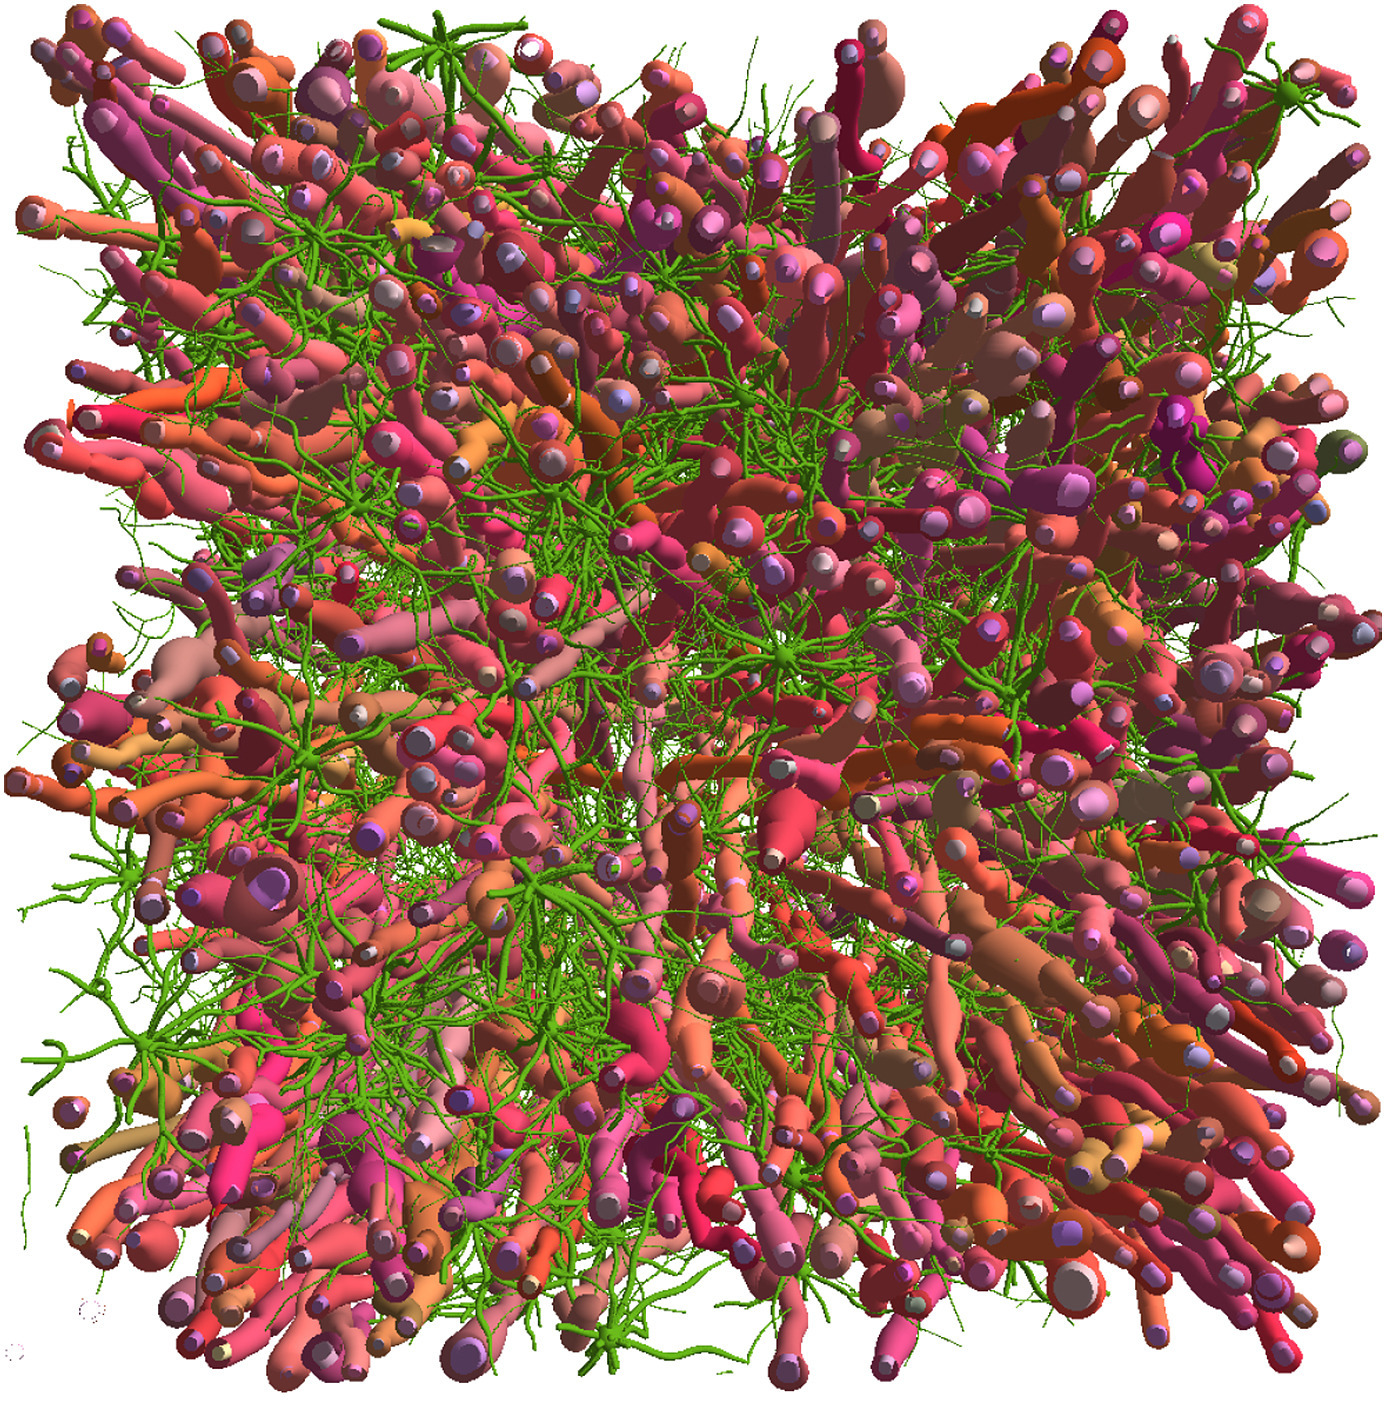
\includegraphics{gfx/model/medusa/11_.jpg}}
	\caption{11 \cite{Ginsburger2019}}
	\label{fig:medusa_11}
\end{figure}
% 
% 
% 
% 
% 
% 
% 
%
% Neurospin works with \ac{dMRI} signals.
% One focus is on the analysis of the fiber architect of the human brain.
% \ac{dMRI} is here quite handy since it is currently the only technique to allow in-vivo measurements to analyse the orientation of white matter tracts. Another importance is the availability of \ac{MRI} machines in almost every hospital in the western civilization.
% Although their resolution is with \SIrange{1.5}{3}{\tesla} limited.
% However, Neurospin is equipped with a mordern \SI{7}{\tesla} \ac{MRI}.
% This makes it possible, including higher measurments times on post mortem brain tissue, a \ac{dMRI} resolution up to \SI{200}{\micro\meter}.
% This makes it possible to allow \ac{3D-PLI} to verify and enhance the analysis of current developed tractography data. 
% %
% Along this works they developed a simulation tool (name) which is computing a Monte-Carlo simulation on the diffusion process in virtual tissues.
% Therefore, for simulations of the \ac{dMRI} signal in the brain, geometric models of nerve fibers as well as nerve cells are required.
% %
% The common goal was, due to a work packes inside the \ac{HBP}, the development of a common general purpose tool to build a geometrical library of nerve fiber configurations.
% Therefore it was decided to work based on the first approaches \cite{Ginsburger2018}.
% %
% \begin{quotation}
% We design a novel white matter numerical phantom generation algorithm which constructs biomimicking geometric configurations with few design parameters, and enables to control the level of disorder of the generated phantoms. The influence of various geometrical parameters present in white matter, such as global angular dispersion, tortuosity, presence of Ranvier nodes, beading, ...
% \end{quotation}
% %
% It is therefore qualified to generate a large database or library of parameter controlled white matter volumes.
% %
% \paragraph{differences:} 
% \begin{itemize}
%     \item All objects are aproximated with spheres.
%     \item Statistical ... of tissue
%     \item diffusion specific parameters
%     \item pathological changes like axon beeding
% \end{itemize}
